%%%%%%%%%%%%%%%%%%%%%%%%%%%%%%%%%%%%%%%%%
% Simple Sectioned Essay Template
% LaTeX Template
%
% This template has been downloaded from:
% http://www.latextemplates.com
%
% Note:
% The \lipsum[#] commands throughout this template generate dummy text
% to fill the template out. These commands should all be removed when 
% writing essay content.
%
%%%%%%%%%%%%%%%%%%%%%%%%%%%%%%%%%%%%%%%%%

%----------------------------------------------------------------------------------------
%	PACKAGES AND OTHER DOCUMENT CONFIGURATIONS
%----------------------------------------------------------------------------------------

\documentclass[12pt]{article} % Default font size is 12pt, it can be changed here
\usepackage{hyperref}
\usepackage{amsmath}
\usepackage{geometry} % Required to change the page size to A4
\geometry{a4paper} % Set the page size to be A4 as opposed to the default US Letter

\usepackage{graphicx} % Required for including pictures

\usepackage{float} % Allows putting an [H] in \begin{figure} to specify the exact location of the figure
\usepackage{wrapfig} % Allows in-line images such as the example fish picture

\usepackage{lipsum} % Used for inserting dummy 'Lorem ipsum' text into the template

\linespread{1.2} % Line spacing

%\setlength\parindent{0pt} % Uncomment to remove all indentation from paragraphs

\graphicspath{{./Pictures/}} % Specifies the directory where pictures are stored
\begin{document}

%----------------------------------------------------------------------------------------
%	TITLE PAGE
%----------------------------------------------------------------------------------------

\begin{titlepage}

\newcommand{\HRule}{\rule{\linewidth}{0.5mm}} % Defines a new command for the horizontal lines, change thickness here

\center % Center everything on the page

\textsc{\LARGE University of Glasgow}\\[1.5cm] % Name of your university/college
\textsc{\Large Human Computer Interaction 4}\\[0.5cm] % Major heading such as course name
\textsc{\large Assessed Exercise}\\[0.5cm] % Minor heading such as course title

\HRule \\[0.4cm]
{ \huge \bfseries Hide and Seek Mobile Application}\\[0.4cm] % Title of your document
\HRule \\[1.5cm]

\begin{minipage}{0.4\textwidth}
\begin{flushleft} \large
\emph{Author:}\\
Garry \textsc{Sharp}\\
0801585s\\ % Your name
\end{flushleft}
\end{minipage}
~
\begin{minipage}{0.4\textwidth}
\begin{flushright} \large
\emph{Supervisors:} \\
Prof. S \textsc{Brewster}\\ % Supervisor's Name
Dr. M \textsc{Chalmers}\\ % Supervisor's Name
Dr. A \textsc{Morrison}\\ % Supervisor's Name
\end{flushright}
\end{minipage}\\[4cm]

{\large \today}\\[3cm] % Date, change the \today to a set date if you want to be precise

%\includegraphics{Logo}\\[1cm] % Include a department/university logo - this will require the graphicx package

\vfill % Fill the rest of the page with whitespace

\end{titlepage}

%----------------------------------------------------------------------------------------
%	TABLE OF CONTENTS
%----------------------------------------------------------------------------------------

\tableofcontents % Include a table of contents

\newpage % Begins the essay on a new page instead of on the same page as the table of contents 

%----------------------------------------------------------------------------------------
%	INTRODUCTION
%----------------------------------------------------------------------------------------

%------------------------------------------------

%\begin{figure}[H] % Example image
%\center{
\includegraphics[width=0.5\linewidth]{placeholder}}
%\caption{Example image.}
%\label{fig:speciation}
%\end{figure}

%----------------------------------------------------------------------------------------
%	MAJOR SECTION 1
%----------------------------------------------------------------------------------------

\section{System Analysis} % Major section

\subsection{Aims of the System}


%------------------------------------------------

\subsection{Usefulness of the System} % Sub-section

%------------------------------------------------

\subsection{Similar Systems} % Sub-sub-section

%\begin{wrapfigure}{l}{0.4\textwidth} % Inline image example
% \begin{center}
%    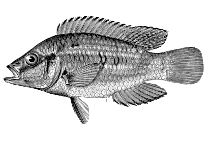
\includegraphics[width=0.38\textwidth]{fish}
%  \end{center}
%  \caption{Fish}
%\end{wrapfigure}
%------------------------------------------------
\newpage
\section{Design and Testing} % Sub-sub-section
\subsection{Design}
\subsubsection{HAPTIMAPS Toolkit}
HAPTIMAPS is an open source toolkit which allows developers to simply and easily create
applications that offer multi-modal feedback for map based applications. Having previously used the
HAPTIMAPS toolkit, I can vouch for its effectiveness and authenticity. This, in fact, was one of
the primary reasons that I decided against its usage in the final system. As native android
provides sufficient functionality for handling GPS data, it was not necessary to include the
HAPTIMAPS toolkit, however, should the app be expanded further (See Section 
\ref{FurtherDevelopment}) I would almost definitly opt to use the toolkit
\subsection{Testing}


\newpage
\section{More Information}
\subsection{Working with new Modalities}

The challenge of working with new modalities was a fun prospect, what added to this was that I was
adament not to use any kind of visual display or feedback, in fact, for the majority of the
implementation stage I kept the android default "Hello World" display (this changed as I now put a
message here if the GPS is not activated). Android offers reasonably good support for accessing the
native vibrate and GPS functions of the mobile device. This meant that applying the application
logic to the vibrate and beep features was relatively straightforward.


\subsubsection{Working with GPS}

One of the initial concerns I had with the system was that of the GPS. Having never used the system
before (accompanied by a limited understanding of how GPS actually works), I did not feel like I
was in the best position to start developing an application that relied heavily upon it. \\

\begin{wrapfigure}{l}{0.5\textwidth} % Inline image example
 \begin{center}
    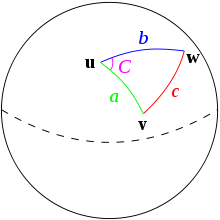
\includegraphics[width=0.42\textwidth]{haversine}
  \end{center}
  \parbox{0.45\textwidth}{\caption{The haversine formula calculating the true distance on the
spherical earth}}
\end{wrapfigure}

After researching the topic, I quickly discovered that many GPS based systems rely heavily upon
maths that is not included as standard in the Java GPS libraries. One such example of this is the
haversine formula which solves the issue of GPS triangulation not giving the true distance between
two points. In reality this is only relevant when calculating distances which are realistically
subject to variation in relation to the curvature of the earth. For instance, calculating distances
over a city would provide a negligable discrpency when constrasting the distances gathered using
the haversine formula with distances caluculated without using it. For this reason, the application
that I have developed does not perform any complex maths using the haversine formula or any other
geo-positioning equations. However, should the app be developed further and used over a
geographical scale, then the app would almost certainly have to feature GPS related maths.

\subsection{Further development}                                                                   
\label{FurtherDevelopment}           
Although the system itself was reasonably simple to implement, especially when faking (to an extent)
some of the back end functionality. What is more interesting here is the broader application of the
multimodal feedback that is received whilst using the app. As the user of a broader system would
only have limited interaction with a GUI, the importance would then be placed on having a system
that accurately conveys meaningful messages via vibration and audio. Currently the feedback
received is of a binary nature, that is to say, in the determination of distance or direction you
judge your accuracy by the presence or lack of a beep/vibration. Currently, it is the intervals
between the beeps and vibrations that indicates to the user their direction and distance. The
initial reason for not providing alternative forms of feedback (for instance different intensity of
vibrations or different audio signals), was that the primary purpose of the app is that of a game.
However, similar systems such as HAPTIMAPS (see above section) allow for users to use a series of
common HCI interactivity modes to give feedback to users using map based applications where the
user cannot see the screen.

\newpage
\section{Conclusion} % Major section

%----------------------------------------------------------------------------------------
%	BIBLIOGRAPHY
%----------------------------------------------------------------------------------------

%\begin{thebibliography}{99} % Bibliography - this is intentionally simple in this template

%\bibitem[Figueredo and Wolf, 2009]{Figueredo:2009dg}
%Figueredo, A.~J. and Wolf, P. S.~A. (2009).
%\newblock Assortative pairing and life history strategy - a cross-cultural
%  study.
%\newblock {\em Human Nature}, 20:317--330.
 
%\end{thebibliography}

%----------------------------------------------------------------------------------------

\end{document}